\section{Project}
\labelsec{Project}
%===========================================================================
\subsection{Database e Altre Rappresentazioni di Dati}

Per la gestione del database si \'e scelto di utilizzare un database NoSql, nell'accezione MongoDB\cite{MongoDB}. In questa sede non si discuteranno i vantaggi, gli svantaggi o le particolarit\'a di questa tecnologia in quanto \'e stato fatto gi\'a ampiamente durante il corso. Di seguito si riportano gli schemi dei documenti che sono stati salvati, le collezioni e il significato di alcuni dei valori inseriti.

\begin{center}
\textbf{Collection Ranges}
\end{center}

In questa collezione di documenti vengono raggruppati tutti i documenti relativi ai ranges che sono da controllare. In particolare sono stati individuati due tipologie di range in base alla tipologia di sensori.

\begin{itemize}
  \item Si/No: Per quella tipologia di sensori che non forniscono effettivamente dei valori ma che notificano solamente la presenza o l'assenza di un particolare elemento come il GAS o il movimento.
  \item  Valore: validi quando un sensore effettivamente serve una misurazione di una grandezza, come ad esempio la temperatura. In questo caso \'e utile sapere se questa grandezza rimane all'interno di determinati range.
\end{itemize}

\begin{figure}[ht]
\centering
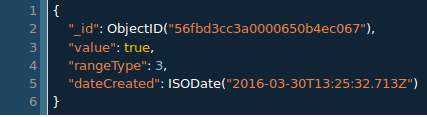
\includegraphics[width=\textwidth,natwidth=610,natheight=642]{Figures/DataStructures/RangesBoolean.png}
\caption{Documento dei Ranges Booleani}
\end{figure}

\begin{figure}[ht]
\centering
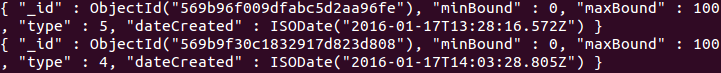
\includegraphics[width=\textwidth,natwidth=610,natheight=642]{Figures/DataStructures/RangesValues.png}
\caption{Documento dei Ranges di Valori}
\end{figure}

Si vuole far notare come sia comunque sempre presente un attributo di tipo data in modo da poter filtrare i range in base al tempo di inserimento e la presenza di un valore numerico che in questo caso rappresenta il tipo di range.

Per indicare il tipo di range si riporta il listato scala che indica tale tipologia.

\begin{figure}[ht]
\centering
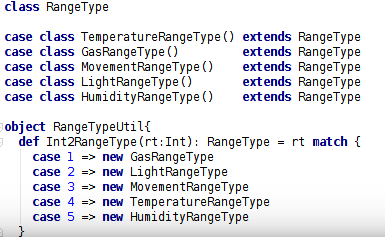
\includegraphics[scale=0.5,natwidth=610,natheight=642]{Figures/DataStructures/Ranges.png}
\caption{Valore numerico dei Ranges}
\end{figure}

\begin{center}
  \textbf{Collertion Sensors}
\end{center}

Per quanto riguarda la collezione dei sensori si utilizza un'apposita collection. Questa non sar\'a modificata spesso, e serve principalmente per eventuali evoluzioni del progetto, in modo che sia gi\'a presente. Anch'essi sono dotati di di tipo come i range e, per questa implementazione, i tipi coincidono. A livello di progetto per\'o si \'e deciso di mantenerli separati nel caso in un futuro questi divergano. Inseriamo di seguito un'immagine che rappresenta come \'e strutturato un documento di un sensore.

\begin{figure}[ht]
\centering
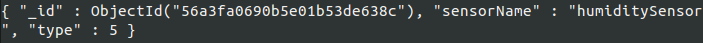
\includegraphics[scale=0.5,natwidth=610,natheight=642]{Figures/DataStructures/Sensors.png}
\caption{Rappresentazione a DB dei Sensori}
\end{figure}

\newpage

\begin{center}
\textbf{Collection Data}
\end{center}

Per quanto riguarda la rappresentazione dei dati raccolti, anche in questo caso sono presenti 2 tipologie di dati, che a loro volta differiscono leggermente per la tipologia di dato, se booleano o meno:
\begin{itemize}
\item Dati Corretti: cio\'e quella tipologia di dati che rientrano all'interno del range prestabilito per la loro tipologia.
\item Dati Incorretti: quelli che invece non rientrano nella tipologia corretta e quindi vanno a violare il range attivo.
\end{itemize}

Come si pu\'o osservare il primo tipo \'e pi\'u semplice in quanto non richiede di salvare anche l'informazione riguardante di quanto il dato risulta errato. Di seguito come fatto in precedenza si indica un esempio di struttura di un dato corretto e non corretto per ogni tipologia di dato.

\begin{figure}[ht]
\centering
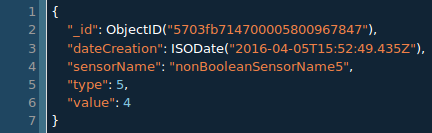
\includegraphics[scale=0.5,natwidth=610,natheight=642]{Figures/DataStructures/DataNoViolation.png}
\caption{Dato Non Booleano Corretto salvato in database}
\end{figure}

Come si pu\'o osservare non \'e stato comunque inserito un valore per la violazione in modo da poter distinguere meglio i dati violati da quelli invece corretti.

\begin{figure}[ht]
\centering
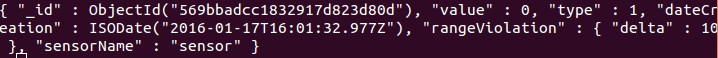
\includegraphics[scale=0.5,natwidth=610,natheight=642]{Figures/DataStructures/DataViolation.png}
\caption{Dato Non Booleano Non Corretto salvato in database}
\end{figure}

In questo caso appunto il valore della violazione non e' piu' nullo ma contiene un semplice campo \textit{delta} che indicher\'a la differenza rispetto al range. In particolare questo sar\'a positivo se il valore registrato supera il range attuale, negativo se invece \'e troppo basso o zero se il tipo di sensoristica e quindi anche di range \'e booleano. Come si puo' vedere nelle seguenti immagini.

\begin{figure}[ht]
\centering
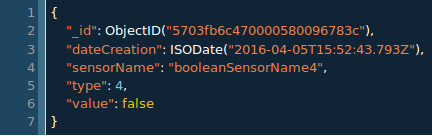
\includegraphics[scale=0.5,natwidth=610,natheight=642]{Figures/DataStructures/BooleanDataNoViolation.png}
\caption{Dato Booleano Corretto salvato in database}
\end{figure}

\begin{figure}[ht]
\centering
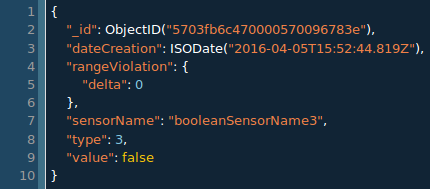
\includegraphics[scale=0.5,natwidth=610,natheight=642]{Figures/DataStructures/BooleanDataViolation.png}
\caption{Dato Non Booleano Non Corretto salvato in database}
\end{figure}

\newpage

\begin{center}
  \textbf{Rappresentazione Dati Attraverso la Rete}
\end{center}

Oltre alla rappresentazione dei dati per quanto riguarda i dati salvati all'interno del Database \'e stato necessario concordare una rappresentazione di dati che verranno inviati attraverso la rete. Non necessariamente le due rappresentazioni devono coincidere in quanto, i dispositivi dai quali si ricavano i dati posso avere diversi formati e modalit\'a di ottenere tali valori, quindi di conseguenza questa rappresentazione \'e sbilanciata rispetto a chi invia i dati, cio\'e il sistema embedded.

Anche per la rappresentazione dei dati si \'e scelta la rappresentazione JSON in quanto questa \'e una delle pi\'u utilizzate nella comunicazione eterogenea via rete, si pone quindi come formato interoperabile tra varie tecnologie, come accade nel nostro caso.

Di seguito si riporta un esempio di dati in formato JSON:

\begin{lstlisting}[language=json]
  {
    "sensorName": "nomeSensore",
    "sensorType": 1,
    "value": true,
    "date": "2016-04-05 17:52:55.058"
  }
\end{lstlisting}

Si veda il tipo di sensore dai valori indicati precedentemente e si sottolinea che il tipo del campo \textit{value} pu\'o essere sia booleano che numerico.

\subsection{Introduzione All'Architettura di Progetto}

Nelle prossime sezioni si vuole inserire le modifiche che sono state fatte alla architettura logica appena introdotta, ma cercando di evitare di ripetere aspetti che non sono effettivamnete cambiati. Di conseguenza si \'e deciso di riportare solamente quegli aspetti che sono stati modificati in base alle scelte tecnologiche effettivamente fatte.\\
In ogni caso si \'e deciso di cercare il pi\'u possibile di sfruttare quanto gi\'a \'e stato concordato dagli analisti cercando di effettuare meno modifiche possibili all'architettura, ma allo stesso tempo di cercare di ridurre le entit\'a che, per ragioni tecnologiche, risultano inutili per la creazione del progetto.

\begin{center}
  \textbf{Server}
\end{center}

\subsection{Struttura}

Vista l'introduzione della tecnologia in questa fase si \'e deciso di apportare alcune modifiche architetturali. Si riporta una lista di modifiche apportate all'architettura:

\begin{itemize}
  \item \textit{DataStructures:} Si \'e ritenuto necessario introdurre un'ulteriore package che non era stato previsto precedentemente contenente le rappresentazioni interne in forma di classi dei dati che circolano nel sistema, cos\'i come delle classi di utilit\'a che servono per la conversione, da e verso, questi dati. (eg . JSON, BSON, DATETIME)
  \item \textit{IDataFormatter:} Visto che le elaborazioni di trasformazione dei dati non richiedono tanta computazione si \'e deciso di eliminare il metodo che, dato un valore lo validava inglobandolo direttamente dentro il primo metodo che restituisce lo stream. Inoltre nella costruzione dello stream ci si \'e accorti che il valore dell'input non viene passato per parametro al metodo, ma viene gestito dall'infrastruttura, quindi si \'e deciso di eliminarlo. Spesso gli oggetti che validano e formattano i dati passano da una rappresentazione ad un'altra: tra valori JSON, BSON e classi interne per i dati.
  \item \textit{IDBDataFormatter:} Viene aggiunto un'ulteriore metodo che gestisce la creazione di dati da un formato inerente alle strutture dati presenti in un altro utilizzabile per lo storage dei dati nel DB. Questo metodo \'e estraneo a quelli per la costruzione di stream e serve per la gestione delle richieste di inserimento di un nuovo range.
  \item \textit{Eliminazione della Maggior Parte dei Formatter:} Questa scelta \'e data dalla possibilit\'a che PlayFramework e altre build in librerie che abbiamo utilizzato consentono per la conversione automatica dei dati da un formato ad un altro, di coseguenza queste operazioni vengono agilmente svolte all'interno del package DataStructures.
  \item \textit{Eliminazione del Presentator:} Anche in questo caso le funzionalit\'a di playframework ci hanno evitato questa implementazione.
  \item \textit{Eliminazione delle Factory:} Visto che la maggior parte delle classi che erano state pensate non inglobano uno stato, ma vengono utilizzate semplicemente per applicare delle computazioni allo stream allora sono state eliminate la maggior parte delle factory class. Grazie anche alla tecnologia scelta (scala) molte delle classi sono state convertite in objects (build-in singletons).
  \item \textit{Eliminazione della classe Configurator:} Si \'e deciso di eliminare tale classe in quando non \'e pi\'u possibile pensare a un entry point per l'applicazione, ma questa viene risvegliata attraverso chiamate rest e di conseguenza molti dei processi legati alla creazione di oggetti \'e stata ridotta.
  \item \textit{Eliminazione del Data Analisys:} A fronte delle semplici operazioni di analisi sui dati (Min, Max, Average) si \'e decisodi sfruttare direttamente le capacit\'a forniteci dal database.
\end{itemize}

\subsection{Interazione}

In questa parte si riporta la tecnologia che si \'e utilizzata per effettuare l'interazione che si \'e analizzata e indicata in fase di analisi, lo stream. In particolare si \'e notato che, il framework play\cite{PlayFramework} gi\'a gestisce attraverso delle sue strutture la possibilit\'a di operare attraverso stream di dati. Questa possibilit\'a \'e stata introdotta dal framework per gestire meglio dati parziali o casi che richiederebbero molto tempo, come ad esempio un'upload di file cospiquo. Nonostante tutto per\'o questo rientra nelle nostre necessit\'a e quindi ci avvarremo di questa astrazione per risolvere il nostro problema. Si riporta in bibliografia quindi la documentazione del framework che spiega il funzionamento di \textit{Enumerators,Iteratees e Enumeratees.} \cite{PlayStreaming}

Un'ulteriore modifica che va apportata visto che ci si trova in ambito web e si dispone di questo framework \'e la necessit\'a di eliminare alcune entit\'a previste precedentemente perch\'e, in fase realizzativa sono risultate ridondanti, ad esempio:
\begin{itemize}
\item \textbf{NewRangeDataReceiver:} Viene rimpiazzato dal controller che gestisce direttamente le richieste POST al sistema per la gestione dei dati provenienti dai form HTTP. Sar\'a questo componente, chiamato \textit{RangeEntryPoint} a validare direttamente i dati in arrivo e a chiamare poi gli elementi successivi nel flusso di dati per il salvataggio di un nuovo range. Si veda l'analisi del problema.
\end{itemize}

\subsection{Comportamento}

\begin{center}
  \textbf{Sistema Embedded}
\end{center}

\subsection{Struttura}
\subsection{Interazione}
\subsection{Comportamento}
